%%%%%%%%%%%%%%%%%%%%%%%%%%%%%%%%%%%%%%%%%
% Texas A&M University Physics Template
% This template has been downloaded from:
% http://www.LaTeXTemplates.com
%
% Modified by Joe Becker
%
% License:
% CC BY-NC-SA 3.0 (http://creativecommons.org/licenses/by-nc-sa/3.0/)
%
%%%%%%%%%%%%%%%%%%%%%%%%%%%%%%%%%%%%%%%%%

%----------------------------------------------------------------------------------------
%	PACKAGES AND THEMES
%----------------------------------------------------------------------------------------

\documentclass{beamer}

\mode<presentation> 

\usetheme{Madrid}
\usecolortheme{dolphin}
\usefonttheme{professionalfonts}

\setbeamertemplate{navigation symbols}{} 

\setbeamertemplate{footline}
{
\leavevmode%
\hbox{%
    \begin{beamercolorbox}[wd=.333333\paperwidth,ht=2.25ex,dp=1ex,center]{section in head/foot}%
        \usebeamerfont{author in head/foot}\insertshortauthor \ {(\insertshortinstitute)}
    \end{beamercolorbox}%
    \begin{beamercolorbox}[wd=.333333\paperwidth,ht=2.25ex,dp=1ex,center]{section in head/foot}%
        \usebeamerfont{title in head/foot}\insertshorttitle
    \end{beamercolorbox}%
    \begin{beamercolorbox}[wd=.333333\paperwidth,ht=2.25ex,dp=1ex,right]{section in head/foot}%
        \usebeamerfont{date in head/foot}\insertshortdate{}\hspace*{2em}
    \end{beamercolorbox}}%
    \vskip0pt%
}

\setbeamertemplate{frametitle}
{
    \begin{beamercolorbox}[sep=0.3cm,ht=1.8em,wd=\paperwidth]{frametitle}
        \vbox{}\vskip-0.0ex%
        \strut\insertframetitle\strut
        \hfill
        \vskip-2.8ex%
    \end{beamercolorbox}
}

\definecolor{maroon}{RGB}{25,25,112}

\setbeamercolor{title}{bg=maroon, fg=white}
\setbeamercolor{block title}{bg=maroon, fg=white}
\setbeamercolor{block body}{bg=maroon!05, fg=black}
\setbeamercolor{frametitle}{fg=maroon, bg=white}
\setbeamercolor{item}{fg=maroon}
\setbeamercolor{section in head/foot}{bg=maroon, fg=white}


\usepackage{graphicx}
\usepackage{booktabs}
\usepackage{textpos} 
\usepackage{media9}
\usepackage{natbib}


%----------------------------------------------------------------------------------------
%	TITLE PAGE
%----------------------------------------------------------------------------------------

\title[ECEN Seminar]{Quantum-memory-assisted Multi-photon Generation for Efficient Quantum Information Processing}

\author[J. Becker]{Joe Becker}

\institute[Texas A\&M]{Texas A\&M Department of Physics and Astronomy

\medskip
\textit{jbecker@physics.tamu.edu} 
}

\date{September 29, 2017} 

\titlegraphic{
\includegraphics[height=2.5cm]{Images/TAMU_logo.png}}

%----------------------------------------------------------------------------------------
% PRESENTATION SLIDES
%----------------------------------------------------------------------------------------

\begin{document}
\setbeamertemplate{items}[circle]

\begin{frame}
\titlepage 
\end{frame}

\begin{frame}\frametitle{Single Photon Sources}
    \begin{center}
        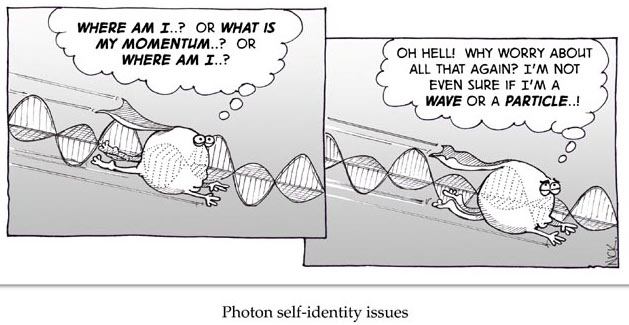
\includegraphics[width=0.7\textwidth]{Images/Photon.jpg}

        \tiny{Cartoon by Nick Kim}
    \end{center}
    Most quantum optics experiments are dependent on having a reliable sources of single photons.
        \begin{itemize}
            \item Photon entanglement and interferometry
            \item Optical quantum computers
            \item Quantum cryptography
        \end{itemize}
\end{frame}


\begin{frame}\frametitle{Single Photon Sources}
    Solid state single photon sources
    \begin{columns}
        \column{0.45\textwidth}
            \begin{block}{Quantum Dots}
                \centering
                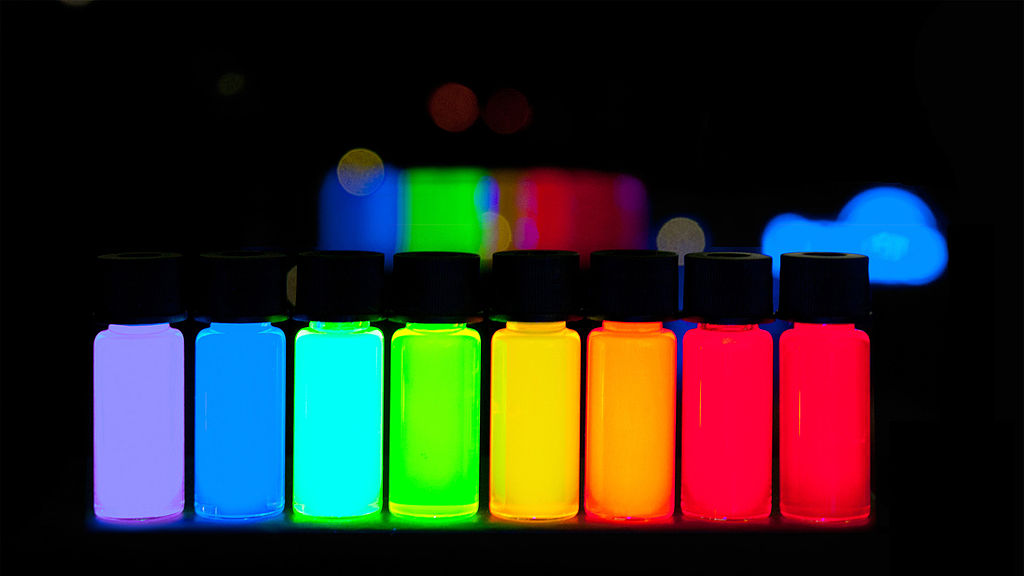
\includegraphics[width=1.0\textwidth]{Images/QuantDots.jpg}

                \tiny{Photo by Wikipedia}
            \end{block}
        \column{0.45\textwidth}
            \begin{block}{Nitrogen-Vacancy Diamonds}
                \centering
                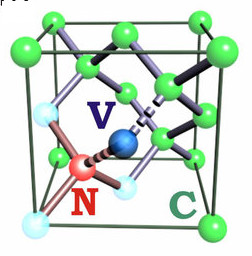
\includegraphics[width=0.6\textwidth]{Images/NVDiamond.jpg}
            \end{block}
    \end{columns}
    \begin{block}{Downsides}
        \begin{itemize}
            \item Requires cryogenic temperatures
            \item Source inhomogeneity
            \item Difficult to achieve high-efficiency photon collection
        \end{itemize}
    \end{block}
\end{frame}

\begin{frame}\frametitle{Single Photon Sources}
    \begin{block}{Spontaneous Parametric Down-conversion}
        \begin{columns}
        \column{0.45\textwidth}
            \begin{itemize}
                \item Uses a $\chi^2$ non-linearity to generate a photon pair from a single high energy pump photon.
            \end{itemize}
        \column{0.45\textwidth}
            \centering
            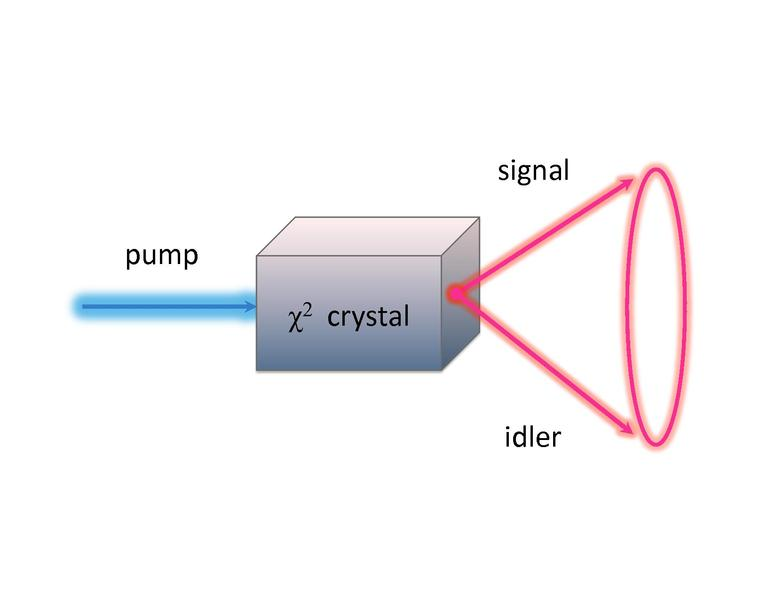
\includegraphics[width=1.0\textwidth]{Images/SPDC.jpg}

            \tiny{Photo by Wikipedia}
        \end{columns}
    \end{block}
    \begin{block}{Downsides}
        \begin{itemize}
            \item Non-Deterministic
            \item Does not scale to multiple coincident photons easily
        \end{itemize}
    \end{block}
\end{frame}

\begin{frame}\frametitle{Multiple Coincident Photon Source}
    Many quantum information applications require many photons
    \begin{block}{Example Experiment: 10 Photon Entanglement}
        \begin{columns}
        \column{0.3\textwidth}
            \begin{itemize}
                \item Using 5 SPDC crystals to generate 10 entangled photons
                \item Coincident rate on the order of an hour
            \end{itemize}
        \column{0.65\textwidth}
            \centering
            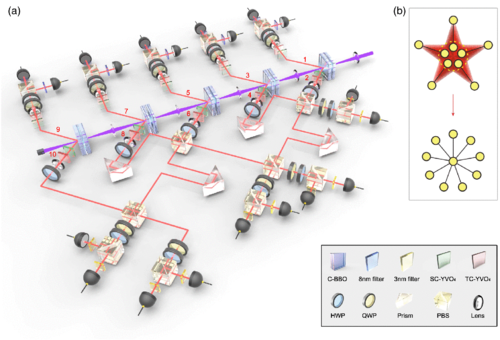
\includegraphics[width=1.0\textwidth]{Images/10Photon.png}

            \tiny{Wang et al. [2016]}
        \end{columns}
    \end{block}
\end{frame}

\begin{frame}\frametitle{Multiple Coincident Photon Source}
    Synchronization of photons of non-local SPDC sources 
    \begin{block}{Example Experiment: Quantum Key Distribution}
        \begin{columns}
        \column{0.55\textwidth}
            \begin{itemize}
                \item Alice and Bob send qubit-encoded photons to Charlie 
                \item Charlie measure correlation through a Bell-state measurement
                \item Increased statistics increases security
            \end{itemize}
        \column{0.4\textwidth}
            \centering
            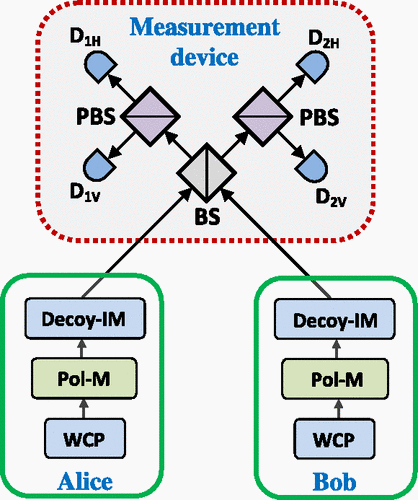
\includegraphics[width=1.0\textwidth]{Images/QKD.png}

            \tiny{Lo et al. [2012]}
        \end{columns}
    \end{block}
\end{frame}

\begin{frame}{Solution: Use quantum memory to assist SPDC sources}
    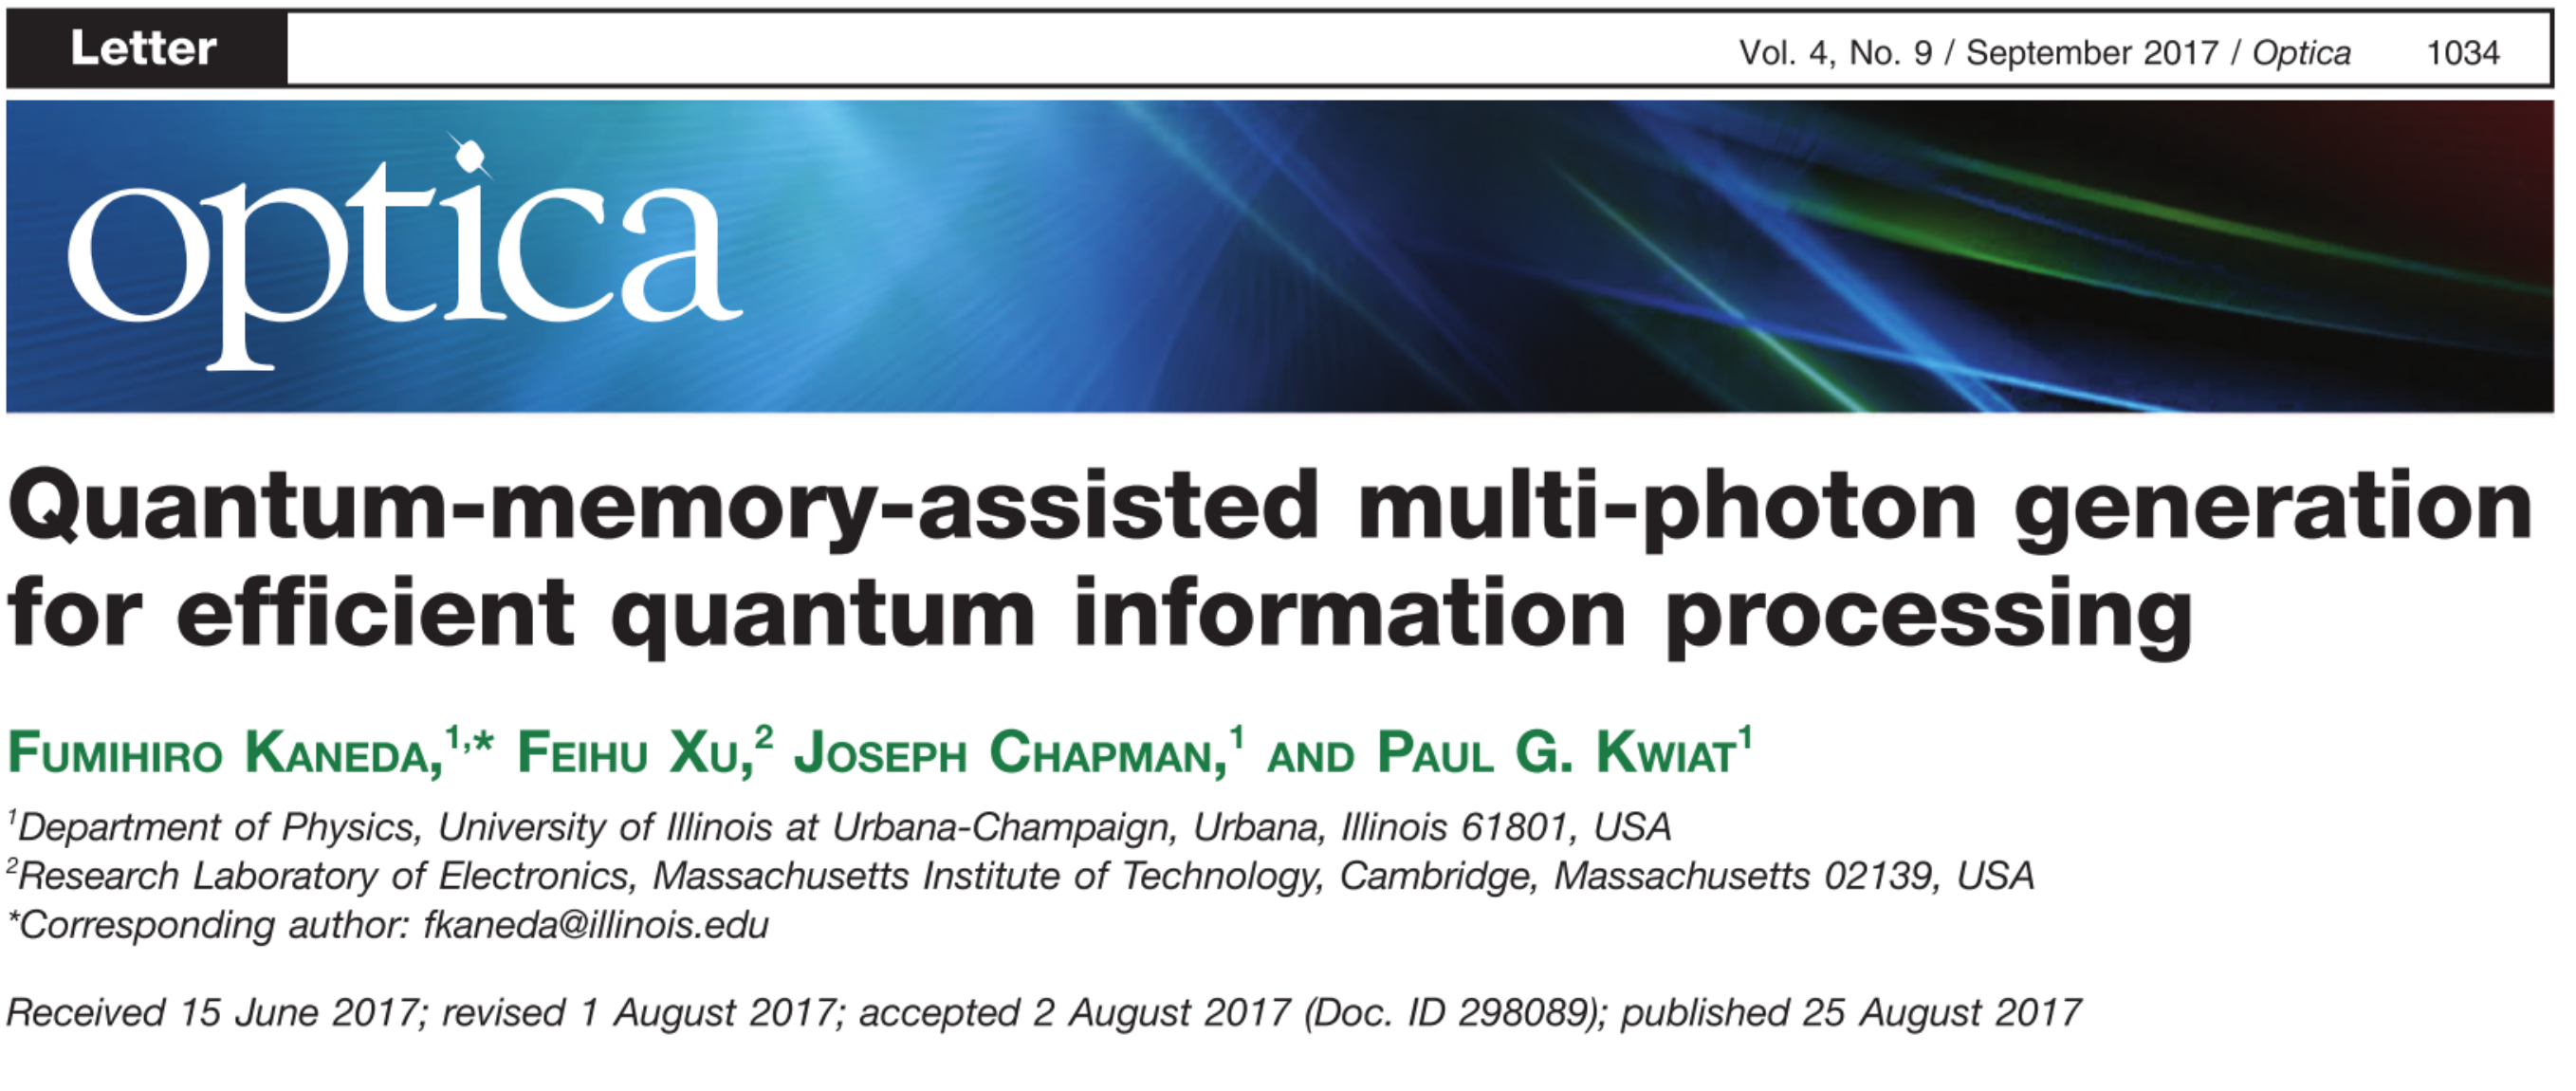
\includegraphics[width=1.0\textwidth]{Images/PaperTitle.png}
\end{frame}

\begin{frame}\frametitle{Quantum Memory}
    \begin{block}{What is a Quantum Memory?}
        \begin{columns}
        \column{0.4\textwidth}
            \begin{itemize}
                \item A conventional memory stores data ($10110101$) for to be recovered at a later time.
                \item A quantum memory stores a quantum state ($|10110101\rangle$) for a time so that it can be later read
            \end{itemize}
        \column{0.5\textwidth}
            \centering
            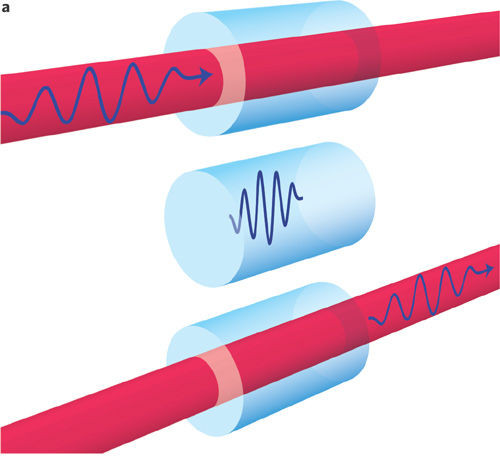
\includegraphics[width=1.0\textwidth]{Images/QuantMem.jpg}

            \tiny{Lvovsky et al. [2009]}
        \end{columns}
    \end{block}
\end{frame}

\begin{frame}\frametitle{Quantum Memories with a Heralded Single Photon Source}
    \centering
    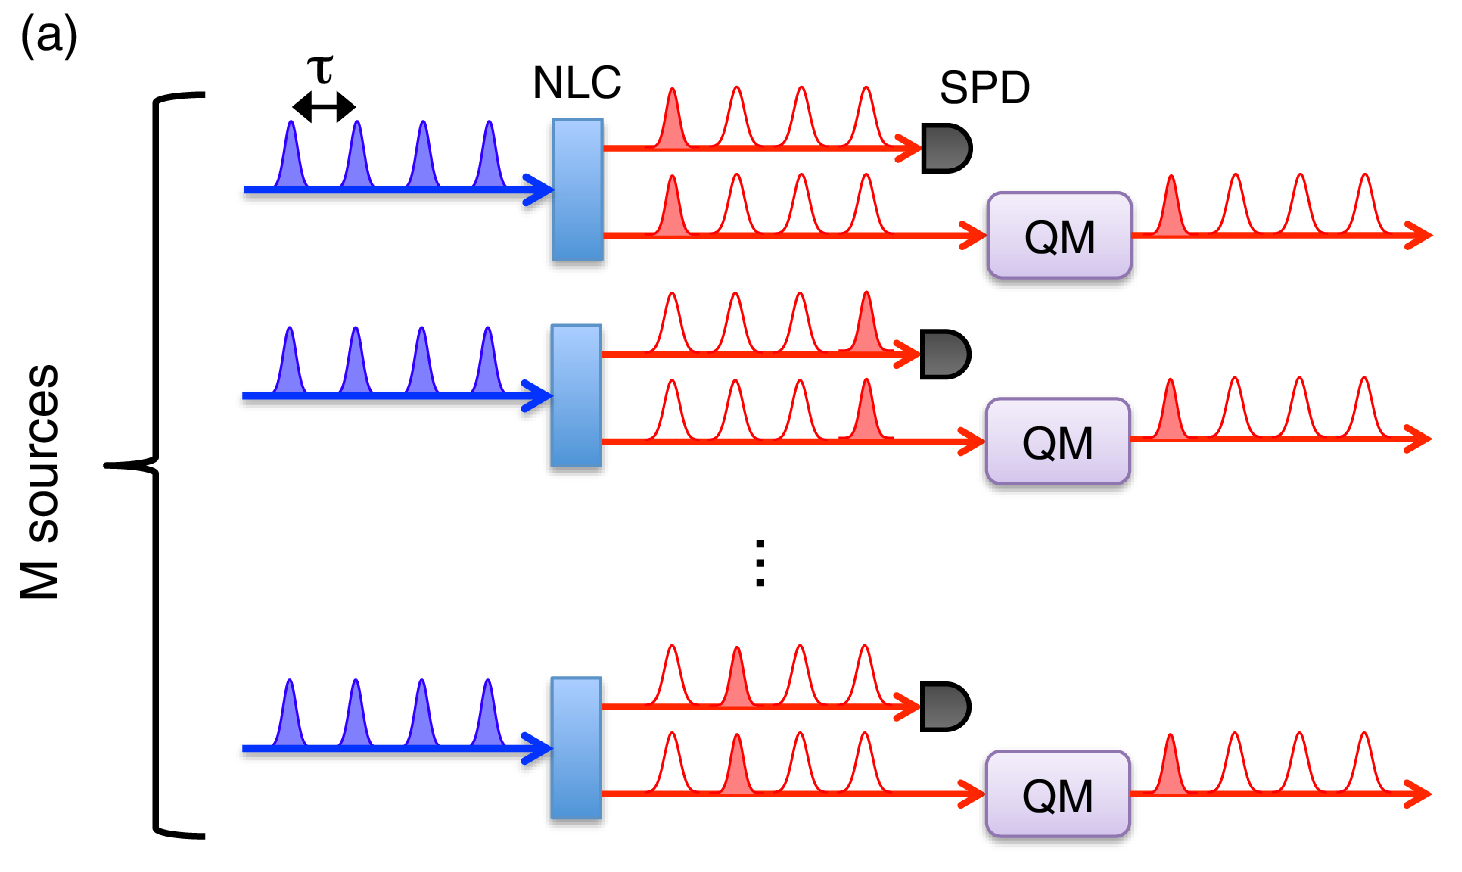
\includegraphics[width=0.9\textwidth]{Images/CoInSchem.jpg}

    \tiny{Kaneda et al. [2017]}
\end{frame}

\begin{frame}\frametitle{Quantum Memories integrated into Quantum Key Distribution}
    Proof of concept application
    \centering
    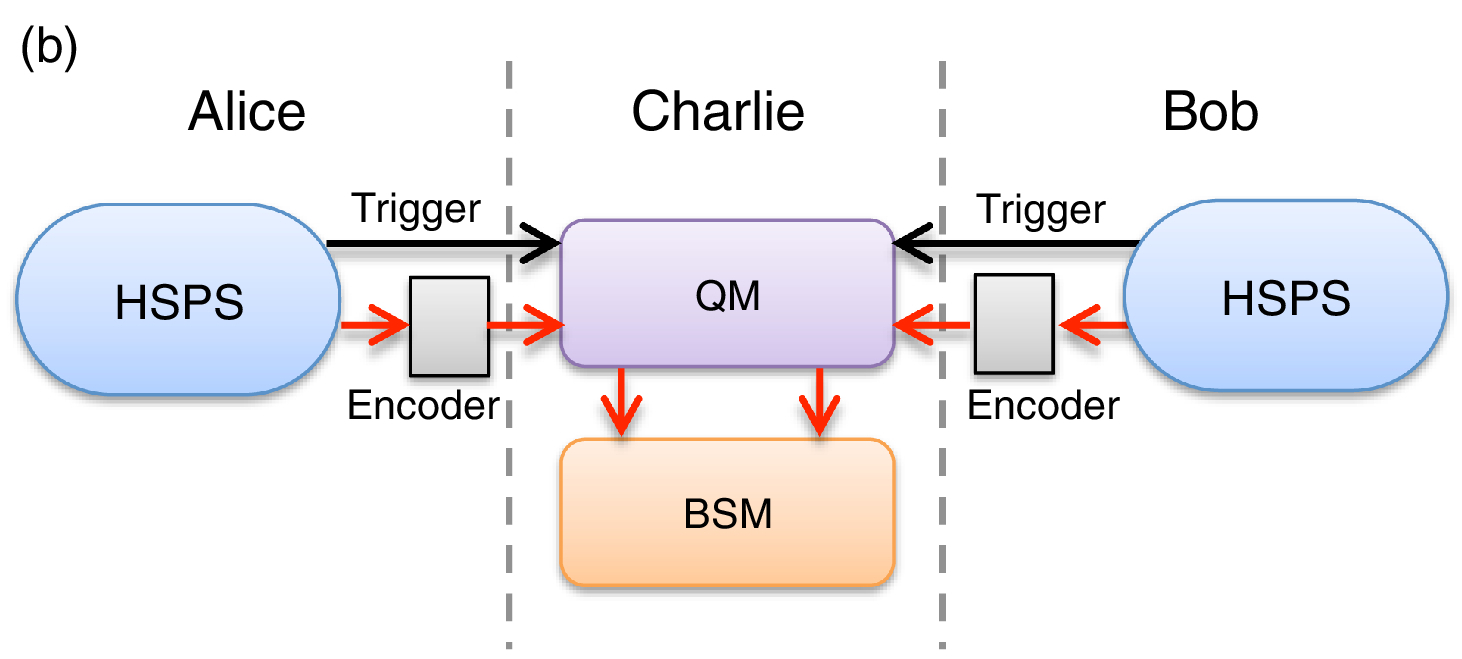
\includegraphics[width=0.9\textwidth]{Images/QMQKD.jpg}

    \tiny{Kaneda et al. [2017]}
\end{frame}

\begin{frame}\frametitle{Experimental Schematic}
    \centering
    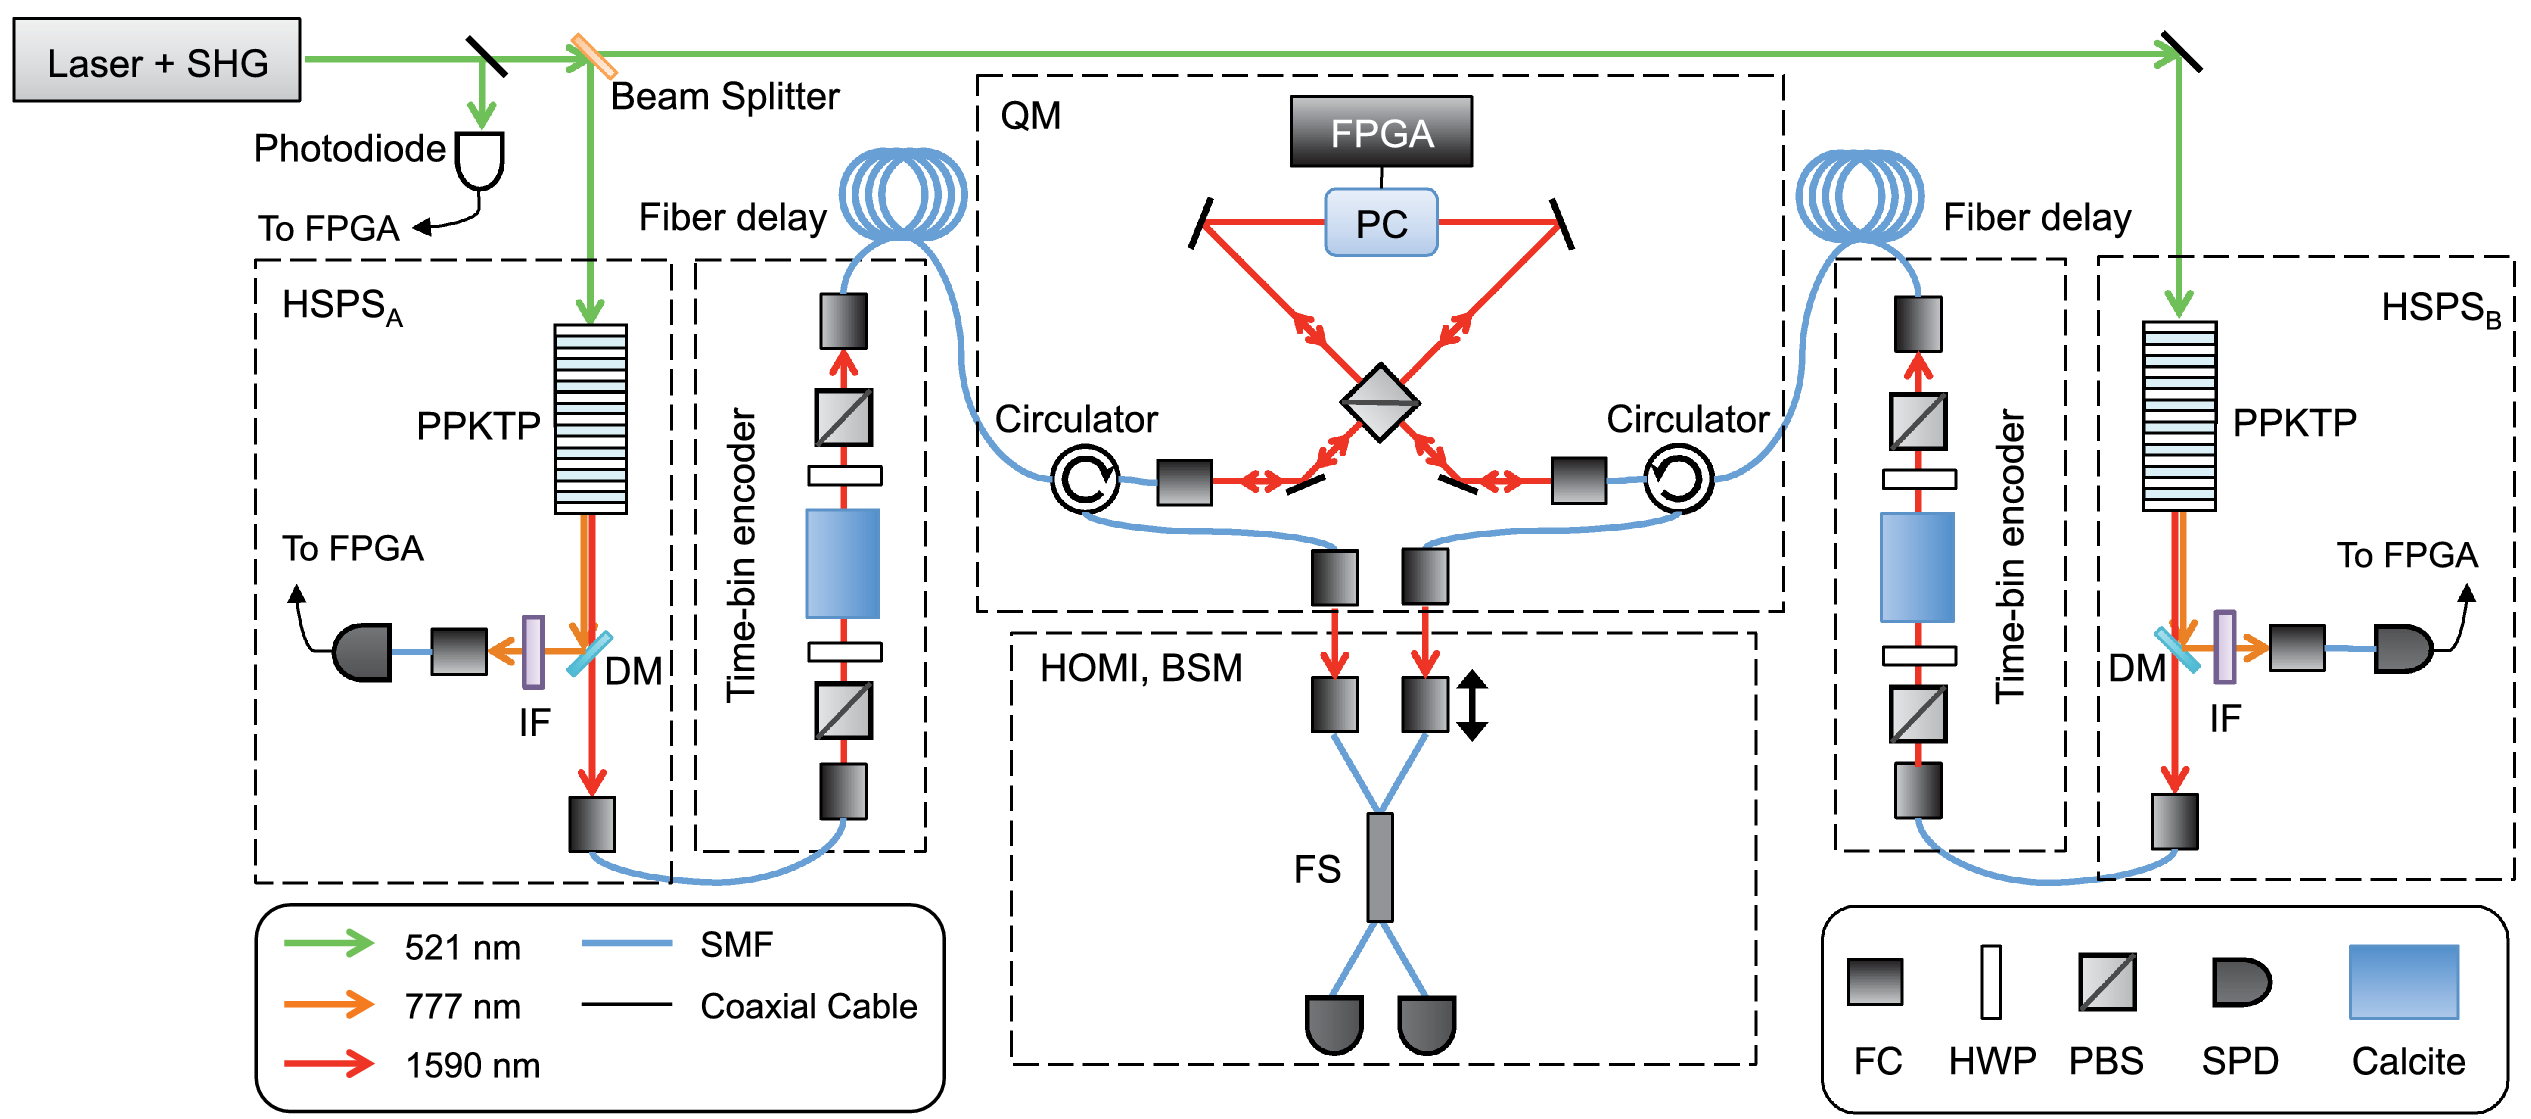
\includegraphics[width=1.0\textwidth]{Images/Figure2.jpg}

    \tiny{Kaneda et al. [2017]}
\end{frame}

\begin{frame}\frametitle{Bulk Optics Quantum Memory Schematic}
    \begin{columns}
    \column{0.3\textwidth}
        \begin{itemize}
            \item Polarized beam splitter allows for storage of photons from two sources
            \item Rubidium titanyl phosphate crystal pair form Pockels cell (PC) to store and release photons
        \end{itemize}

    \column{0.7\textwidth}
    \begin{center}
    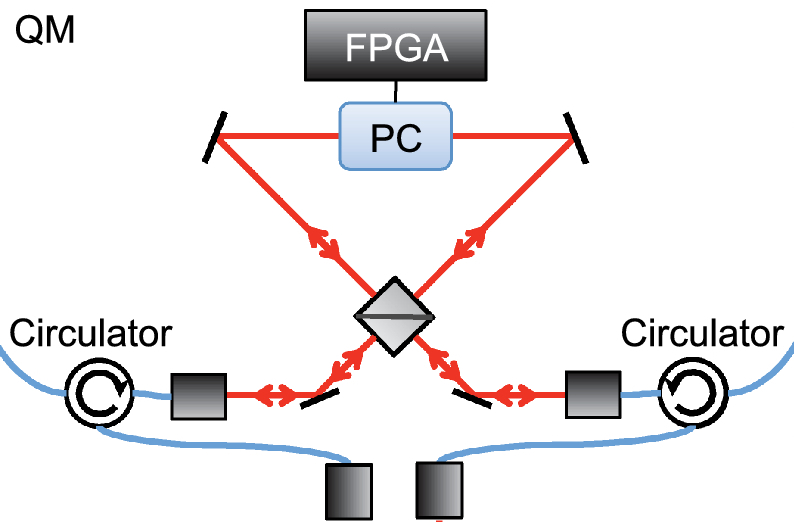
\includegraphics[width=1.0\textwidth]{Images/QMSchem.jpg}

    \tiny{Kaneda et al. [2017]}
    \end{center}
    \end{columns}
\end{frame}

\begin{frame}\frametitle{Coincidence Counts}
    \centering
    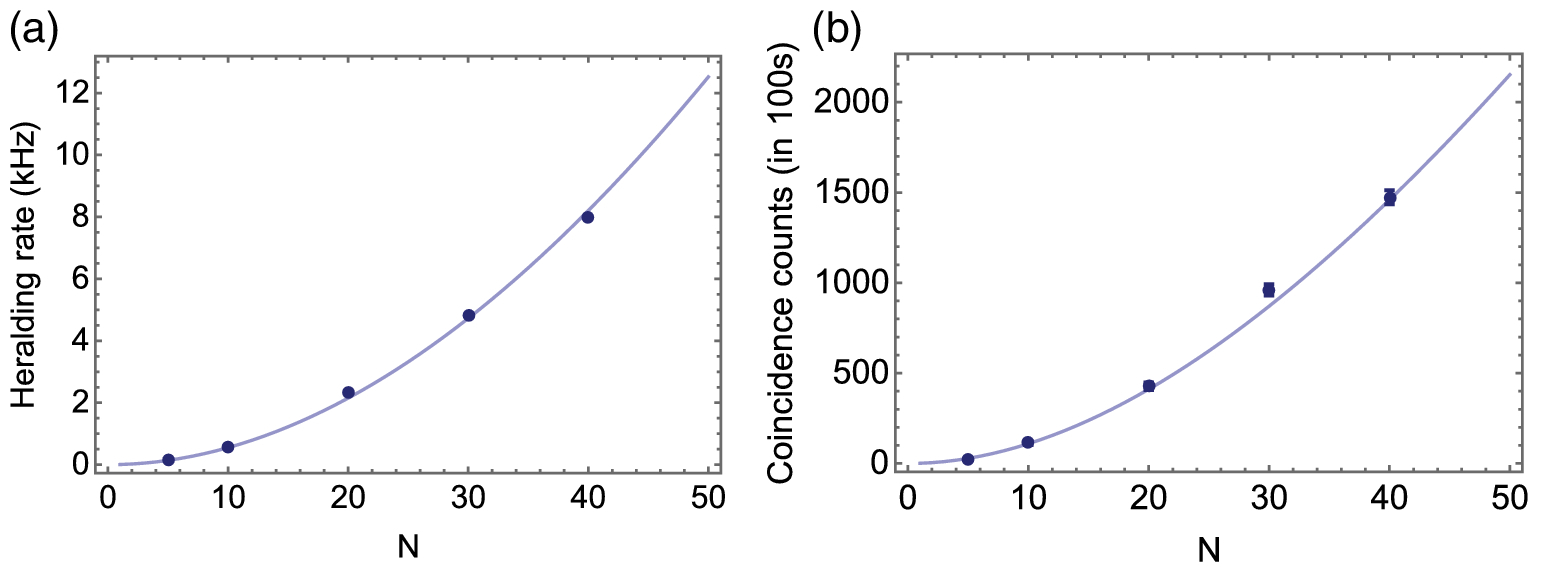
\includegraphics[width=0.8\textwidth]{Images/Figure3a.jpg}

    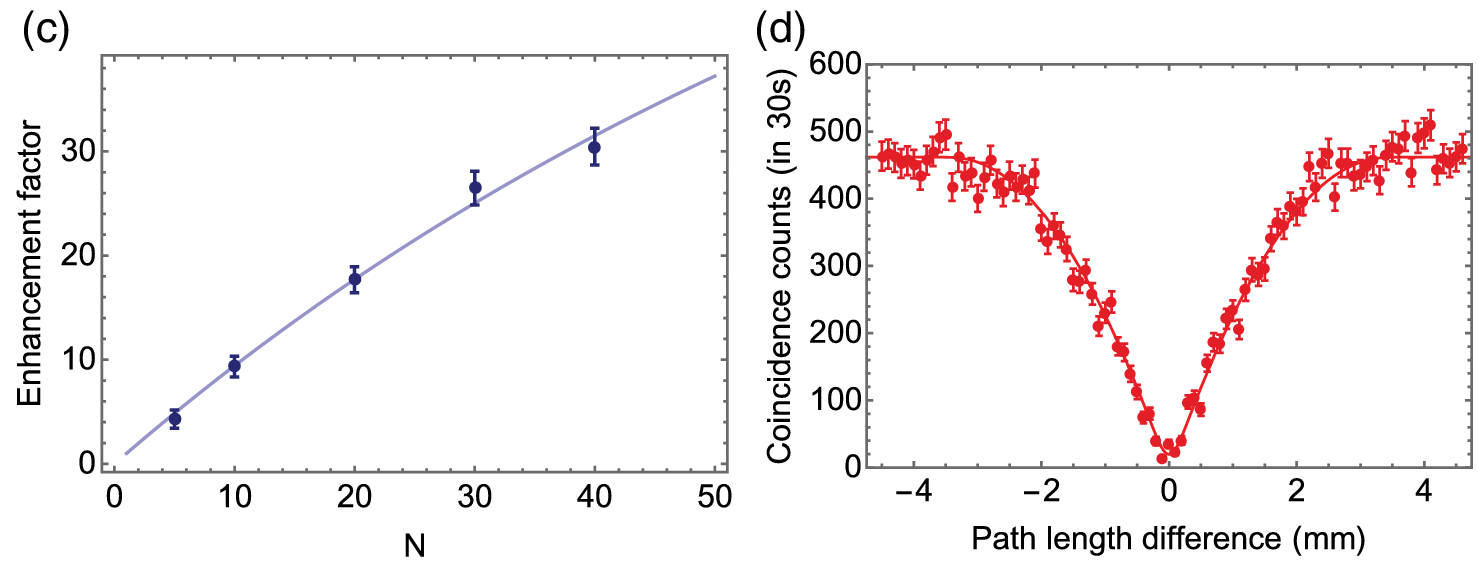
\includegraphics[width=0.8\textwidth]{Images/Figure3b.jpg}

    \tiny{Kaneda et al. [2017]}
\end{frame}

\begin{frame}\frametitle{Hong-Ou-Mandel Interference as BSM}

    \begin{center}
    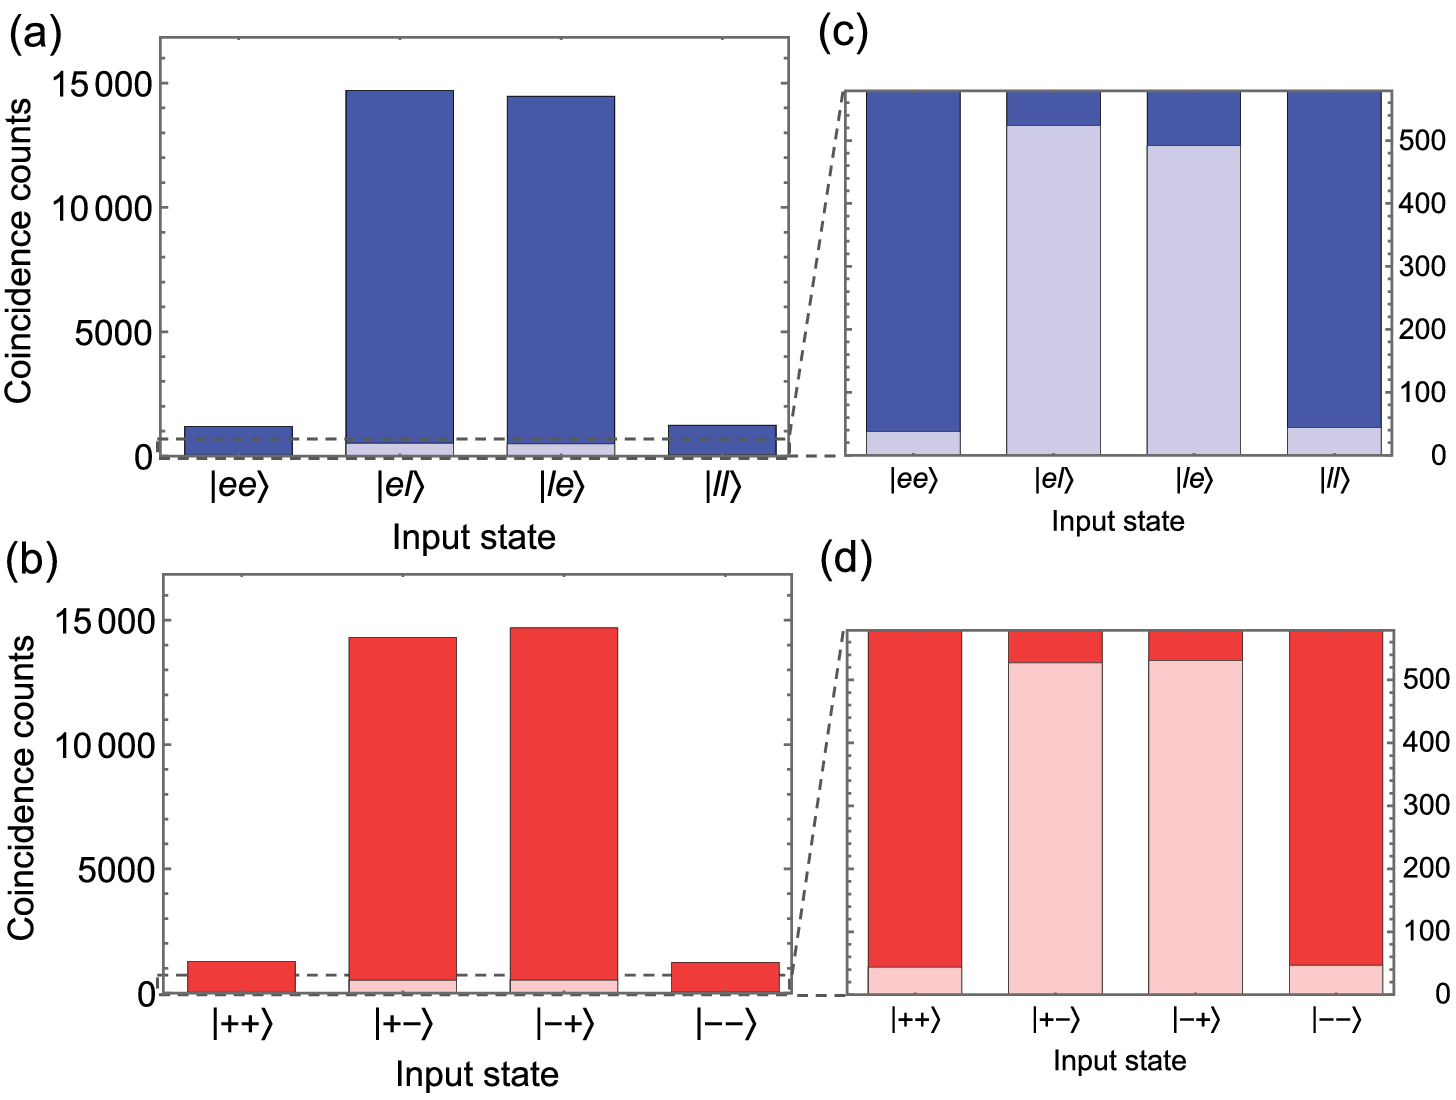
\includegraphics[width=0.75\textwidth]{Images/Figure4.jpg}

    \tiny{Kaneda et al. [2017]}
    \end{center}
\end{frame}


\begin{frame}{Conclusions}
    \begin{itemize}
        \item Integration of the quantum memory enhanced coincidence rate by $30$
        \item The current set up could be extended to allow for generation of up to 10 synchronized single photons 
            with a generation rate of $\gtrsim1\ s^{-1}$.
        \item Reduction of optical loss could make up to 30 coincident photons every few seconds a possibility.
    \end{itemize}
\end{frame}

\end{document}

